\documentclass[10pt,a4paper]{article} %rozmiar czcionki i klasa dokumentu
\usepackage[left=1.5cm, right=1.5cm]{geometry} %szerokosc marginesu
\usepackage[utf8]{inputenc} 
% \usepackage[latin2]{inputenc} ten pakiet gryzie się z powyższym i poniższym!
\usepackage[polish]{babel} %dolacza pakiet z jezykiem polskim 
% \usepackage{polski} alternatywny pakiet
\usepackage[T1]{fontenc} %poprawne składanie polskich czcionek
\usepackage{indentfirst} %pierwszy akapit wciety

\usepackage{graphicx,subfigure}
\usepackage{psfrag}
\usepackage{wrapfig}

\graphicspath{{./obrazki/}}

\usepackage{amsmath}
\usepackage{amsfonts}
\usepackage{array}
\usepackage{supertabular}
\usepackage{array}
\usepackage{tabularx}
\usepackage{hhline}

\usepackage{listings}
\usepackage{xcolor}

\definecolor{codegreen}{rgb}{0,0.6,0}
\definecolor{codegray}{rgb}{0.5,0.5,0.5}
\definecolor{codepurple}{rgb}{0.58,0,0.82}
\definecolor{backcolour}{rgb}{0.95,0.95,0.92}

\lstdefinestyle{selfstyle}{
	backgroundcolor=\color{backcolour},   
	commentstyle=\color{codegreen},
	keywordstyle=\color{magenta},
	numberstyle=\tiny\color{codegray},
	stringstyle=\color{codepurple},
	basicstyle=\ttfamily\footnotesize,
	breakatwhitespace=false,         
	breaklines=true,                 
	captionpos=b,                    
	keepspaces=true,                 
	numbers=left,                    
	numbersep=5pt,                  
	showspaces=false,                
	showstringspaces=false,
	showtabs=false,                  
	tabsize=2
}

\lstset{style=selfstyle}
\begin{document}
\title{Projektowanie Algorytmów i Metod Sztucznej Inteligencji \\
	   \large Algorytmy Sortowania}
\author{Dawid Krekora 254003}
\date{\today}
\maketitle
\tableofcontents
	\newpage
	\section{Wprowadzenie}
	Potrzeba implementacji algorytmów sortowania nastała wraz z rozwojem technologicznym. Przy ogromnej ilości wszechobecnych danych, ręczne dopsowywanie elementów do zadanego klucza byłoby operacją czasochłonną i niepozbawioną błędów wynikających z dokładności pracy ludzkiej. Dlatego też opracowano narzędzia pomocnicze które miały za zadanie temu pomóc - a sam wybór algorytmu zależał już od rodzaju problemu który napotkamy.
	\section{Opis badanych algorytmów sortowania}
	\subsection{Sortowanie przez scalanie}
	Sortowanie przez scalanie (ang. merge sort) jest typowym reprezentantem metody "dziel i zwyciężaj". Algorytm jest podzielony na 3 główne części:
	\begin{itemize}
		\item dzielenie głównego problemu na dwie równe części
		\item wywołanie rekurencyjne sortowania przez scalanie dla każdej z nich
		\item połączenie posortowanych elementów w całość
	\end{itemize}
	Klasa obliczeniowa sortowania przez scalanie jest taka sama dla każdegj złożoności problemu i wynosi $ O (n log n) $ co oznacza, że nasz algorytm jest wydajnym algorytmem którego czas wykonania przyrasta dużo wolniej od np. wzorostu kwadratowego - który jest mało optymalny jeżeli chcemy uzyskać jak najlepszą wydajność obliczeniową.
	\subsection{Sortowanie szybkie}
	Sortowanie szybkie (ang. quick sort) tak samo jak poprzednik opiera swoje działanie na metodzie "dziel i zwyciężaj". Schemat działania algorytmu wygląda bardzo podobnie do tego w merge sort:
	\begin{itemize}
		\item w losowy sposób wyznaczamy piwot który będzie naszym odnośnikiem do danych w strukturze danych (np. tablicy liczb)
		\item wykonujemy operacje porównań które doprowadzają do podziału tablicy na dwie części: z liczbami mniejszymi od piwota po lewej i większymi po prawej.
		\item wywołujemy procedurę quick sort dla dwóch części tablicy osobno
		\item połączenie posortowanych elementów w całość
	\end{itemize}
	Dużą zaletą quick sorta jest fakt, że w momencie dojścia do momentu połączenia tablic, elementy są już posortowane. Losowe wybieranie piwota niesie jednak ryzyko uzyskania najgorszego możliwego scenariusza - takiego w którym to piwot zawsze będzie wylosowany jako ostatni element tablicy. Powoduje to, że przy średniej złożoności problemu osiągamy klasę złożoności $ O (n log n) $, jednak w najgorszym przypadku musimy liczyć się z kwadratowym przyrostem czasu w stosunku do liczby przetwarzanych elementów: $ O (n^2) $.
	\subsection{Sortowanie przez kopcowanie}
	Sortowanie przez kopcowanie (ang. heap sort) wykorzystuje do swojego działania drzewo binarne typu maksymalnego. To struktura danych w której wyróżniamy z góry określoną relację rodzic-dziecko pomiędzy elementami struktury (rodzic może mieć dwoje dzieci ale dziecko tylko jednego rodzica). I to właśnie ta struktura jest tutaj kluczowa w założeniu tego algorytmu sortowania. Elementy już w momencie umieszczania w kopcu muszą przejść podstawowe procedury sortowania tak, aby było spełnione założenie drzewa binarnego. To zapewnia niezwykle równą i efektywną klasę złożoności dla każdego z przypadków problemów: $ O (n log n) $.
	\clearpage
	
	\section{Przebieg eksperymentów}
	Testowanie algorytów polegało w dużej mierze na sprawdzeniu ich zachowania przy rozwiązywaniu rzeczywistego problemu. Same testy opierały się na mierzeniu czasu trwania sortowania za pomocą konkretnych algorytów:
	\begin{itemize}
		\item w pierwszym etapie przygotowane zostały tablice o różnej wielkości (10000,50000,100000,500000,1000000)
		\item następnie tablice te zostały wypełnione zgodnie z założeniem testu (wszystkie elementy losowe, posortowane ale malejąco lub posortowane w pewnym $ \% $)
		\item dla każdego rozmiaru tablicy i kryterium podstawowego każdy test został przeprowadzony 100 krotnie, mierząc czas wykonania każdego z testu osobno
		\item wyciągnięto średnią z wyników - uzyskano średni czas działania algorytmów
	\end{itemize}
	Poniżej przedstawiono tabele z rezultatami testów dla trzech badanych algorytmów sortowania: 
	\begin{figure}[!ht]
		\centering
		\subfigure[]{%
			\label{fig:Obraz4}%
			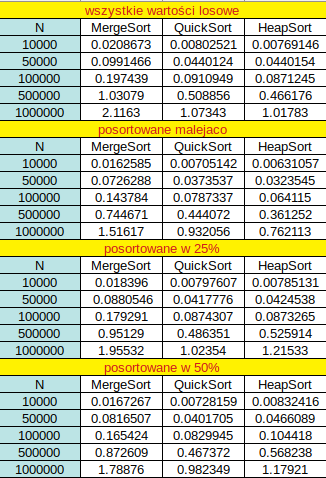
\includegraphics[width=0.4\textwidth]{test1.png}% Suma wszystkich wartości width nie powinna być większa niż 1!
		}
		\subfigure[]{%
			\label{fig:Obraz5}%
			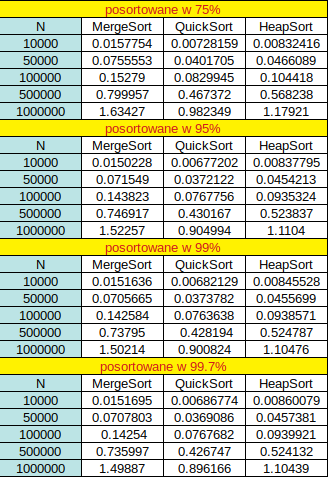
\includegraphics[width=0.40\textwidth]{test2.png}}
		\caption{Rezultaty pracy algorytów - wyniki czasowe.}
		\label{fig:obraz2}
	\end{figure}

	\clearpage
	\section{Podsumowanie i wnioski}
	Tabele pokazane na rysunku (Rysunek 1.) prowadzą do kilku istotnych wniosków:
	\begin{itemize}
		\item Każdy z zaprezentowanych algorytmów, pomimo posiadania złożoności obliczeniowej $ O (n log n) $ posortował tablice w różnym czasie
		\item najsłabiej wypadł algorytm sortowania MergeSort, był on zdecydowanie najwolniejszy od dwóch pozostałych. Wynika to z faktu, że stopień posortowania danych zapewnia mu jedynie brak potrzeby zamiany elementów miejscami. Etap porównań musi w dalszym ciągu przeprowadzić dla całego zakresu tablicy. Najbardziej kosztowna jest jednak ilość porównań które trzeba wykonać ponownie po dojściu do najniższego poziomu wywołania rekurencji
		\item algorytmy quicksort i heapsort rywalizowały ze sobą o miano najszybszego co jest dużym zaskoczeniem ponieważ w uniwersyteckich modelach algorytm heapsort okazywał się najwolniejszym z nich trzech. W naszym przypadku, przy mniejszym rozmiarze problemu, dorównywał quicksortowi, a nawet był od niego szybszy. O ile ten aspekt można wytłumaczyć, np. niekorzystnym rozmieszczaniem piwotu to w żaden sposób nie tłumaczy tak wyraźnej przewagi nad mergesortem.
		\item wniosek końcowy: algorytmy quicksort i heapsort wydają się być zaimplementowane w sposób poprawny, zgodnie z definicją książkową. Algorytm mergesort posiada pewne bliżej nieokreślone różnice w składni, przez co efekt jego działania nie jest idealny
	\end{itemize}
	\section{Literatura}
	\begin{itemize}
		\item "Data Structures and Algorithms in C" - Michael T.Goodrich
		\item "Algorytmy, struktury danych i techniki programowania" - Piotr Wróblewski
		\item www.wikipedia.com
	\end{itemize}
	
	
	
	
	
	


		
\end{document}